\chapter{System Design}
\label{ch:system}

\section{Overview}
\label{sec:system:overview}

Splatt3R-SLAM uses four processes when refinement and the GUI are enabled
(\cref{fig:system-overview}). The \emph{tracker} consumes
frames, runs the feed-forward backbone, solves \cref{eq:gn} for the relative
pose against the current keyframe, and decides when to create a new keyframe.
The \emph{back-end} maintains the keyframe graph, queries retrieval for loop
candidates and solves \cref{eq:global}. The \emph{refiner}
(\cref{ch:refiner}) is optional and photometrically improves the assembled map
while the other two run. The \emph{visualiser} renders the current map and
subscribes to refined snapshots. Both headless experiments and GUI-enabled
dual-GPU delivery measurements are reported, with their regimes identified.
Figure~\ref{fig:method-overview} gives the method path from image pairs to
the refined map; Fig.~\ref{fig:system-overview} gives the process layout.

\begin{figure}[t]
  \centering
  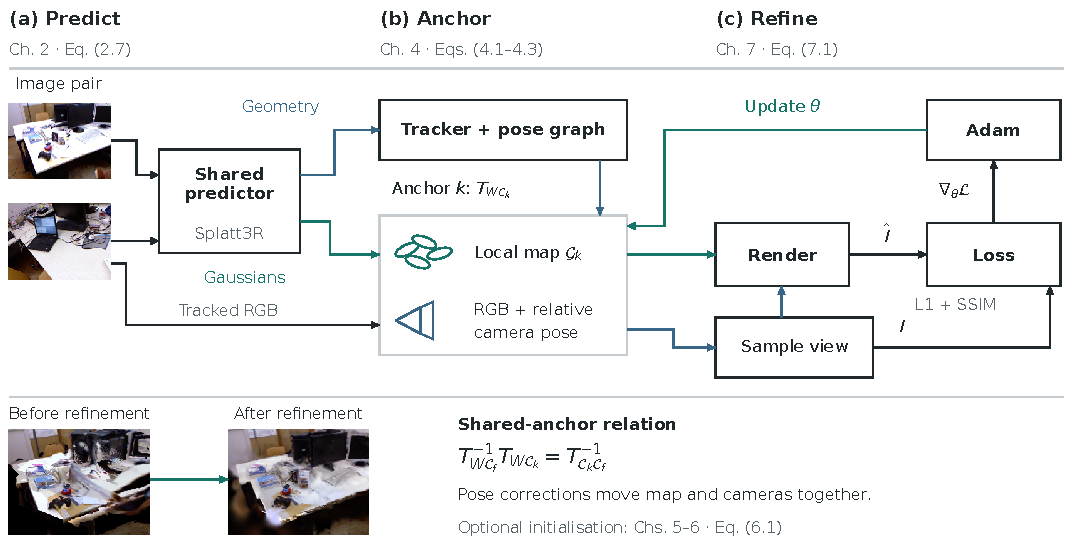
\includegraphics[width=\linewidth]{ral/fig/method_overview_master.pdf}
  \caption[Predict, anchor, and refine]{Method navigation. Real input frames
  enter a shared predictor. Geometry feeds tracking, while local Gaussians
  attach to keyframe anchors. The same anchors carry supervision cameras.
  A separate process samples observations, renders the map, and updates its
  appearance. Chapter and
  equation labels point to the detailed derivation.}
  \label{fig:method-overview}
\end{figure}

The refiner runs in its own process. This allows it to use a different GPU,
which \cref{ch:refiner} shows reduces contention in the measured TUM desk
configuration.
It also separates photometric optimisation from geometric tracking: the
refiner reads the pose state but does not optimise or write tracking poses.
Resource contention can still affect scheduling and end-to-end throughput.

SharedKeyframes stores images, pointmaps, confidences, poses and Gaussian
payloads in CUDA tensors exposed through inter-process communication.
The refiner transfers new Gaussian payloads to its device and reads current
anchor poses. Separately, tracked RGB supervision and anchor-relative camera
transforms live in the CPU SupervisionFrames pool. Complete refined maps are
published through a CPU snapshot buffer. These are distinct storage paths.

\begin{figure}[t]
  \centering
  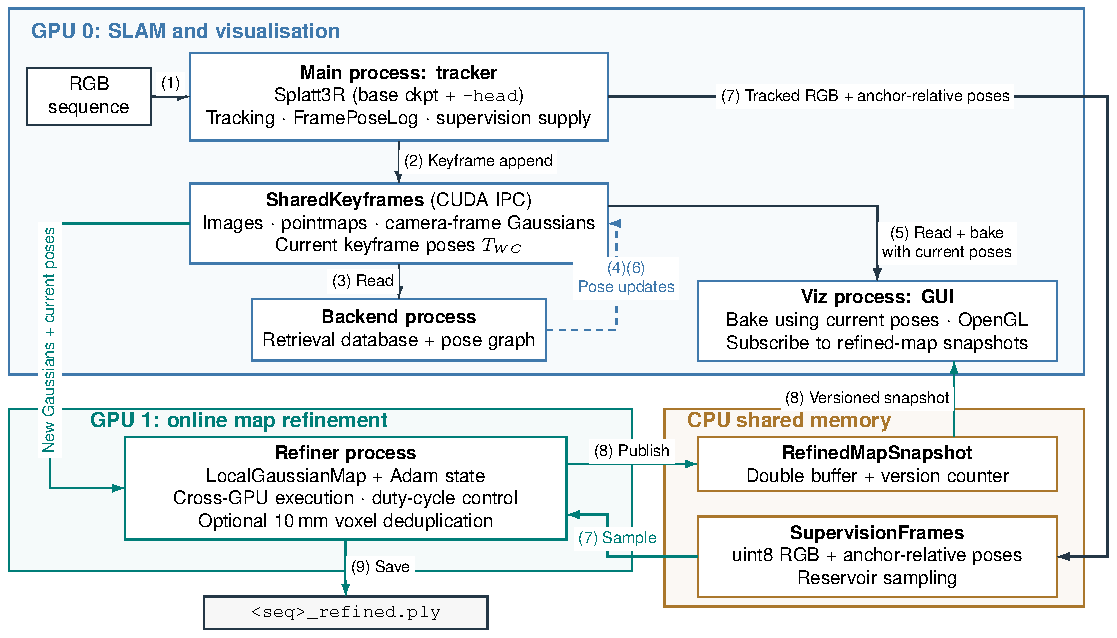
\includegraphics[width=\linewidth]{ral/fig/overview.pdf}
  \caption[System overview]{System overview.
  Tracking, backend optimisation, and visualisation run on GPU~0; the map
  refiner runs on GPU~1. SharedKeyframes uses CUDA IPC, while supervision
  frames and versioned refined-map snapshots use CPU shared memory.
  Numbered arrows show RGB, predicted pointmaps, local Gaussians, supervision
  and refined-map flow; dashed arrows denote pose updates. Thumbnails use
  real TUM desk predictions and recorded maps. Before/after renders share
  one camera; the backend inset shows recorded keyframe camera centres.}
  \label{fig:system-overview}
\end{figure}

\section{Anchor-carried map composition}
\label{sec:system:anchor}
We replace the pointmap prediction with Splatt3R, so each keyframe pair yields
a per-pixel Gaussian in one forward pass. Keyframe Gaussians are stored in
their anchor keyframe's local frame and composed into the world through that
keyframe's \emph{current} pose,
\begin{equation}
\mu_n^{W}=a_kR_k\mu_n^{\mathcal C_k}+t_k,\qquad
\Sigma_n^{W}=a_k^2R_k\Sigma_n^{\mathcal C_k}R_k^\top,
\label{eq:anchor}
\end{equation}
where $T_{W\mathcal C_k}=(a_kR_k,t_k)$ is the camera-to-world
$\mathrm{Sim}(3)$ pose of keyframe $k$. Because the composition reads the
pose at render time, a loop closure that updates $T_{W\mathcal C_k}$ moves
the map without rewriting local parameters.

Supervision uses the same anchor. If tracked frame $f$ stores a relative pose
$T_{\mathcal C_k\mathcal C_f}$, then
\begin{equation}
T_{W\mathcal C_f}
=T_{W\mathcal C_k}T_{\mathcal C_k\mathcal C_f}.
\label{eq:supervisionpose}
\end{equation}
For a local map and camera sharing anchor $k$, their relative transform is
\begin{equation}
T_{W\mathcal C_f}^{-1}T_{W\mathcal C_k}
=(T_{W\mathcal C_k}T_{\mathcal C_k\mathcal C_f})^{-1}
 T_{W\mathcal C_k}
=T_{\mathcal C_k\mathcal C_f}^{-1}.
\label{eq:anchorconsistency}
\end{equation}
The anchor cancels, so any invertible update of $T_{W\mathcal C_k}$ preserves
this relation. The identity applies within one anchor; neighbouring local maps
can still disagree.

The implementation stores means, scales, rotations, SH coefficients, opacity,
confidence, and validity in a shared keyframe buffer. Tracker updates may
rewrite pointmap state without clearing the Gaussian record unless a new
Gaussian prediction is present. This invariant prevents a geometric update
from silently erasing an already renderable keyframe. Filtering and the
global Gaussian limit are applied before rasterisation; the limit is therefore
a rendering budget implemented through spatial stride, rather than FIFO
deletion of individual keyframes.

\section{The injection pipeline}
\label{sec:system:injection}

Between ``the network emitted a Gaussian'' and ``the Gaussian is in the map''
sit several filters, and their order matters because two of them interact with
the contribution of \cref{ch:thin}.

\begin{enumerate}\itemsep3pt
\item \textbf{Validity.} Pixels without a valid pointmap prediction emit no
      Gaussian.
\item \textbf{Confidence gate.} Gaussians below \texttt{--refiner-min-confidence}
      are dropped outright. This is a \emph{deletion} operation and is
      deliberately kept distinct from thinning, which is not.
\item \textbf{Scale clamp.} An optional cap on injected scale, applied at
      refinement time and independent of the bake-time cap, bounds the damage a
      single mispredicted $\hat{s}$ can do to a render.
\item \textbf{Band-limiting.} Injected Gaussians are optionally band-limited
      against the measured lattice pitch of the prediction grid
      (\texttt{--refiner-aa-sigma}), which removes the dot/moir\'e pattern that
      a per-pixel Gaussian field otherwise produces when viewed off-axis.
\item \textbf{Opacity thinning.} \Cref{eq:thin}, the subject of
      \cref{ch:thin}.
\end{enumerate}

The global Gaussian limit is applied \emph{before} rasterisation and is
implemented as a spatial stride over the map, not as FIFO deletion of
keyframes. The distinction is not cosmetic: a FIFO policy would make the
displayed map a function of how long the sequence has been running, whereas a
stride makes it a function of the display budget alone, and leaves the
evaluation artefact --- the full map, written to disk --- untouched by whatever
the viewer could afford to draw.

\section{Rendering, display and the evaluation artefact}
\label{sec:system:render}

The refiner publishes a versioned snapshot in CPU memory rather than exposing
mutable GPU state. The visualiser uploads only complete versions and retains
the previous valid version if it collides with a write. If the display buffer
is smaller than the refined map, publication subsamples --- but only after the
full map has been saved. This ordering means a failure to publish a large map
for display cannot discard a valid refinement result, which is a failure mode
we hit before separating the two paths.

On termination the system writes the refined map as a standard 3DGS
\texttt{.ply}, so that it can be scored, inspected or rendered by any tool in
that ecosystem rather than only by ours. The external rendering comparisons
in \cref{ch:results} use these artefacts and the full-SH evaluation script.
Earlier component ablations use the recorded map-scoring harness for their
respective paired runs. Neither uses viewer screenshots as quantitative data.

\section{Changes to MASt3R-SLAM}
\label{sec:system:diff}

We replace the pointmap
prediction with Splatt3R's joint pointmap-and-Gaussian prediction; we add the
Gaussian record to the shared keyframe buffer; we add the injection pipeline
of \cref{sec:system:injection}; and we add the refiner process of
\cref{ch:refiner}. We change nothing in matching (\cref{eq:trackray}), nothing
in keyframe selection, nothing in the retrieval path, and nothing in the
back-end solver (\cref{eq:global}).

The one place where this could leak is the pointmap itself, since Splatt3R and
MASt3R share an encoder and decoder but the fine-tuned head is ours. Head-only
training (\cref{ch:adapt}) keeps the encoder and decoder bit-frozen, so the
pointmap the tracker consumes is bit-identical to what MASt3R would have
produced. This is why \cref{sec:exp:ate} reports parity rather than
improvement; it serves as a control for the inherited tracking path.
